\documentclass[12pt]{article}
\usepackage[brazil]{babel}
\usepackage[a4paper, total={6.5in, 9.5in}]{geometry}
\usepackage[utf8]{inputenc}
\usepackage[T1]{fontenc}
\usepackage{listings}
\usepackage{xcolor}
\usepackage{float}
\usepackage{graphicx}
\usepackage{hyperref}
\usepackage{lipsum}
\usepackage[normalem]{ulem}

\definecolor{codegreen}{rgb}{0,0.6,0}
\definecolor{codegray}{rgb}{0.5,0.5,0.5}
\definecolor{codered}{rgb}{0.8,0,0}
\definecolor{backcolour}{rgb}{0.95,0.95,0.92}

\usepackage{inconsolata}
\lstset{
    language=sql,
    backgroundcolor=\color{backcolour},   
    commentstyle=\color{codegreen},
    keywordstyle=\color{blue},
    numberstyle=\tiny\color{codegray},
    stringstyle=\color{codered},
    basicstyle=\ttfamily\small,
    numberstyle=\footnotesize,
    numbers=left,
    backgroundcolor=\color{gray!10},
    frame=single,
    tabsize=2,
    rulecolor=\color{black!30},
    title=\lstname,
    escapeinside={\%*}{*)},
    breaklines=true,
    breakatwhitespace=true,
    framextopmargin=2pt,
    framexbottommargin=2pt,
    inputencoding=utf8,
    extendedchars=true,
    showstringspaces=false,
    literate={á}{{\'a}}1 {ã}{{\~a}}1 {é}{{\'e}}1 {Ó}{{\'O}}1 {Ã}{{\~A}}1 {í}{{\'i}}1 {ó}{{\'o}}1,
}

\title{Atividade Views e Procedures}
\author{Pedro Henrique de Brito Agnes, 18/0026305 \\
Pedro Pessoa Ramos, 18/0026488}
\date{19 de Novembro de 2020}

\begin{document} 
\maketitle

\section*{View}
Foi criada uma view para o projeto final para listar todas as pessoas cadastradas no banco, unindo as tabelas de alunos e professores.

\begin{lstlisting}
create view pessoas as
select 'aluno', nome, email from aluno
union all
select 'professor', nome, email from professor
order by nome;

-- select * pessoas
\end{lstlisting}

\begin{figure}[H]
	\centering
    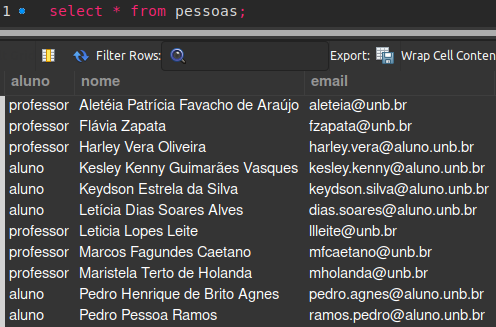
\includegraphics[width=.8\textwidth]{pessoas.png}
    \caption{Resultado do select na view}
\end{figure}

\section*{Procedure}
Foi criada uma procedure para o banco de dados desenvolvido no projeto final com o objetivo de computar pontos extras para alunos com a pontuação acima da média.

\begin{lstlisting}
DELIMITER //

CREATE PROCEDURE professorLegal(IN Turma VARCHAR(2), IN Diciplina VARCHAR(8))
BEGIN
    DECLARE done INT DEFAULT FALSE;
    DECLARE aluno VARCHAR(9);
    DECLARE nota FLOAT;
    DECLARE mediaTurma FLOAT;
    DECLARE curs1 CURSOR FOR 
    (
        SELECT par.aluno_matricula, SUM(tip_par.pontuacao * par.tempo) FROM participacao AS par 
        INNER JOIN tipo_participacao AS tip_par ON par.tipo_participacao_id = tip_par.id
        WHERE par.aula_turma_id = Turma AND par.aula_turma_disciplina_codigo = Diciplina
        GROUP BY par.aluno_matricula
    );
    DECLARE CONTINUE HANDLER FOR NOT FOUND SET done = TRUE;
    SET mediaTurma = (
        SELECT AVG(tip_par.pontuacao * par.tempo) 
        FROM participacao AS par 
        INNER JOIN tipo_participacao AS tip_par ON par.tipo_participacao_id = tip_par.id
        WHERE par.aula_turma_id = Turma AND par.aula_turma_disciplina_codigo = Diciplina
        GROUP BY par.aula_turma_id
    );
    OPEN curs1;
        read_loop: LOOP
            FETCH curs1 INTO aluno, nota;
            IF done THEN
                LEAVE read_loop;
            END IF;
            IF nota > mediaTurma THEN
                INSERT INTO participacao (aluno_matricula, tipo_participacao_id, aula_numero, aula_turma_id, aula_turma_disciplina_codigo) SELECT aluno,"1",A.numero, A.turma_id, A.turma_disciplina_codigo from aula as A WHERE A.turma_id = Turma AND A.turma_disciplina_codigo = Diciplina LIMIT 1;
            END IF;

        END LOOP;
    CLOSE curs1;


END //

DELIMITER ;

-- CALL professorLegal('A','CIC0124');
\end{lstlisting}

\begin{figure}[H]
	\centering
    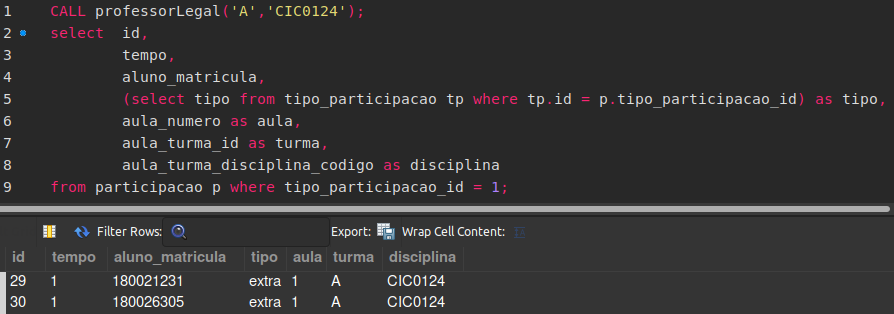
\includegraphics[width=1\textwidth]{professor_legal.png}
    \caption{Resultado do select na tabela de participações após executar a procedure}
\end{figure}

\end{document}
